\author{Esben Pilgaard Moeller}

\section{Scalability}
\begin{frame}{Scalability}{}
\begin{block}{Scalability Issues}
  \begin{itemize}
  	\item Design handles scalability issues with drones, not users
    \item An increasing amount of users will result in an increased load on the server
    \item We assume an increased amount of users will result in:
    \begin{itemize}
			\item More page loads (Computation)
			\item More privileges which are loaded often when using the system (Computation and I/O)
			\item More session key requests
		\end{itemize}
		\item Scaling with hardware or software
  \end{itemize}
\end{block}
\end{frame}

\subsection{Hardware}
\begin{frame}{Scalability}{Hardware}
  \begin{columns}[T]
    \begin{column}{.5\textwidth}
     \begin{block}{}
% Your text here
    \begin{itemize}
  	\item Uses a Master/slave architecture
    \item Scale-out on Master to handle increased load
    \item Scale-out and apply use a distributed database to distribute I/O operations  
    \item Session keys requests could be distributed accross physical machines
    \end{itemize}
    \end{block}
    \end{column}
    \begin{column}{.5\textwidth}
    \begin{block}{}
% Your image included here
    \begin{center}
    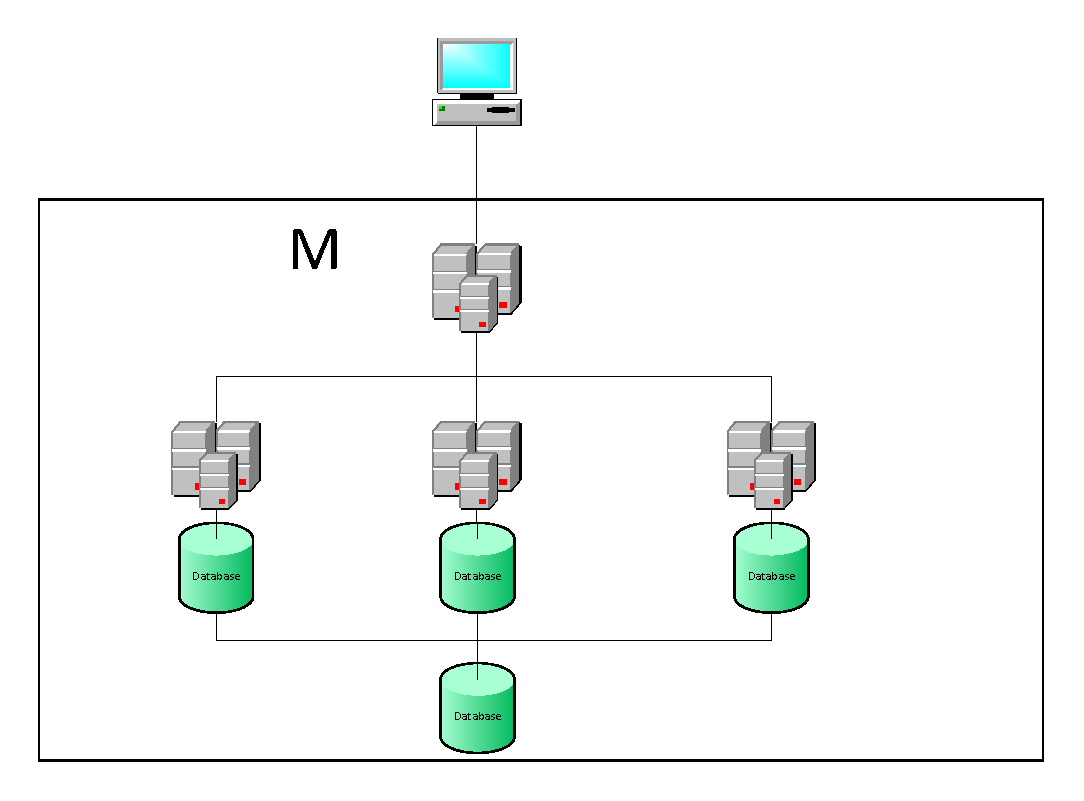
\includegraphics[width=0.7\textwidth]{images/master_scaling.pdf}
    \end{center}
    \end{block}
    \end{column}
\end{columns}\end{frame}



\subsection{Software}
\begin{frame}{Scalability}{Software}
  \begin{itemize}
    \item Caching and Replicas
    \item Can be applied on both the application and DB level
  \end{itemize}
\end{frame}

\begin{frame}{Scalability}{Software}
\begin{block}{Application level}
  \begin{itemize}
    \item Scale-out on Master and use two identical application servers
    \begin{itemize}
			\item Can use shared DB or DB replicas 
		\end{itemize}
    \item Perform usage analysis and cache frequently accessed pages 
  \end{itemize}
\end{block}
\end{frame}

\begin{frame}{Scalability}{Software}
\begin{block}{Caching on DB level}
  \begin{itemize}
    \item Cache frequently accessed DB records
    \item Cache the results of frequently posed querries
    	\begin{itemize}
				\item Rails stores results of querries for the duration of an action 
			\end{itemize}
		\item Creates issues with consistency
  \end{itemize}
\end{block}
\end{frame}